%---------------------------%
\section{August 2021} %---%
%---------------------------%
% \addcontentsline{toc}{section}{August 2021}

%%%%%%%%%%%%%%%%%%%%%%%%%%%%%%%%%%%%%
\subsection*{Classical Mechanics} %%%
%%%%%%%%%%%%%%%%%%%%%%%%%%%%%%%%%%%%%
\addcontentsline{toc}{subsection}{Classical Mechanics}

\prob{1.1}{

A Lagrangian for a system with infinitely many interacting particles of mass $m$ (infinitely many degrees of freedom, $-\infty < n < +\infty$) is given as follows:
\begin{align*}
    \mathcal{L} = \sum_{n=-\infty}^{\infty} \Big[ \frac{m}{2} \dot{x}_n^2 - \frac{k}{2} (x_n - x_{n-1})^2 \Big]
\end{align*}

\begin{parts}
    \item What kind of system does this Lagrangian describe?

    \item Write down the Lagrangian equations of motion.

    \item Show that there is a solution given by $x_n(t) = A \cos(\omega t - c n)$.

    \item Find an equation for $c$

    \item For $c \ll 1$, find the approximate magnitude of $c$.
    What kind of motion does the solution describe?
    What is the interpretation of the constant $c$?
\end{parts}

}

\sol{}


\prob{1.2}{

Two bars of equal masses $m$ connected by a weightless spring can slide with no friction along a horizontal $xy$-plane.
The bars are initially at rest but at time $t > 0$ a constant horizontal force $f$ is applied to the left bar, as shown in the Figure.
The spring has the stiffness $k$ and the length $l$ in undeformed state.

\begin{parts}
    \item Write down the Lagrangian in terms of the center of mass coordinate $Q(t)$ and the distance $u(t) = x_2(t) - x_1(t)$ between the bars, assuming that they move only along the $x$-axis.
    Here $x_1(t)$ and $x_2(t)$ are the coordinates of the left and the right bars, respectively.

    \item Solve the equations of motion for $Q(t)$ and $u(t)$ with the initial conditions $x_1(0) = 0$, $x_2(0) = l$, and $\dot{x}_1(0) = \dot{x}_2(0) = 0$, where the overdot means the time derivative.

    \item Find the amplitude and the frequency of oscillations of the distance between the bars $u(t)$ at $t > 0$.
\end{parts}

\begin{center}
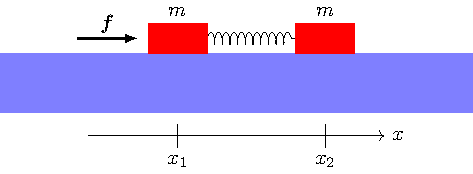
\includegraphics{August2021/1-2.pdf}
\end{center}

}

\sol{}


\prob{1.3}{

A spherical pendulum consists of a particle of mass $m$ in a gravitational field constrained to move on the inner surface of a sphere of radius $R$.

\begin{parts}
    \item Use the polar angle $\theta$ (measured from the downward vertical) and the azimuthal angle $\phi$ as generalized coordinates and obtain the Hamiltonian.
    Are there any conserved quantities?

    \item Obtain the equations of motion in the Hamiltonian formulation.

    \item Assume the particle performs uniform circular motion with $\theta$ fixed at $\theta_0$.
    What are the values of the constants of motion (if any) in such a case?
\end{parts}

}

\sol{}


\prob{1.4}{

\begin{parts}
    \item Calculate the escape velocity $v_e$ from the surface of a homogeneous sphere of density $\rho$ and radius $R$,

    \item A vertical shaft extends to the center of a homogeneous sphere of density $\rho$ and radius $R$ and a small mass is dropped from rest at the surface.
    Compare the velocity attained at the center with the escape velocity.

    \item Suppose the sphere is not homogeneous but the density $\rho(r)$ is a function of the distance to the center.
    Find $\rho(r)$ for which the mass falls to the center with constant acceleration.
\end{parts}

}

\sol{}


\prob{2.1}{

A harmonic oscillator with a spring constant $k$ and mass $m$ is damped with a force $-bv$ where $v$ is the velocity of the mass and $b$ is a constant.
The mass is also driven by a harmonic force $F(t) = F_0 \cos{\omega t}$.

Given $F_0$, at what angular frequency $\omega$ the amplitude of the displacement is maximal?

}

\sol{}

%%%%%%%%%%%%%%%%%%%%%%%%%%%%%%%%%%%%%%%%%%
\subsection*{Electricity \& Magnetism} %%%
%%%%%%%%%%%%%%%%%%%%%%%%%%%%%%%%%%%%%%%%%%
\addcontentsline{toc}{subsection}{Electricity \& Magnetism}


\prob{2.2}{

The region bounded by two concentric spherical surfaces with radii $R_1$ and $R_2$ ($R_1 < R_2$) is filled with a charge density $\rho = \alpha / r$.

Find the total charge $Q$ and spatial distribution of the electrostatic potential $\Phi(\vb*{r})$ and the electric field $\vb*{E}(\vb*{r})$.

For a fixed total charge $Q$, consider the behaviors of $\Phi(\vb*{r})$ and $\vb*{E}(\vb*{r})$ in the limit of an infinitely thin spherical shell, i.e., $R_1 \rightarrow R_2$.

}

\sol{}


\prob{2.3}{

The plane $z = 0$ carries a charge such that the potential on that plane is $\Phi(x,y,0) = V_0 \sin{k x}$.

Find the potential everywhere in space.

}

\sol{}


\prob{2.4}{

It is believed that Compton scattering by starlight quanta may be a mechanism for the energy degradation of high-energy electrons in interstellar space.
An experiment has been proposed in which this phenomenon can be observed directly in the laboratory by scattering a high-energy electron beam against the intense flux of visible photons produced by a typical laser.
The experimentalists have established that the laboratory energy of the scattered photon is given to an excellent approximation ($\beta \approx 1$) by the relation
\begin{align*}
    E_f^{\gamma} \approx \gamma m c^2 \frac{\lambda ( 1 - \beta \cos{\theta_0} )}{1 + \lambda ( 1 - \cos{\theta_0} )}, \quad \lambda = 2 \gamma \frac{E_i^{\gamma}}{m c^2}
\end{align*}
where $E_i^{\gamma}$ is the laboratory energy of the incident photon, $\theta_0$ is the photon scattering angle in the electron rest frame, $m$ is the electron mass, $c$ is the speed of light, and $\gamma = (1 - \beta^2)^{-1/2}$.
Having joined the experiment, you are asked to verify that this relation is correct.
In order to do so, proceed as follows:

\begin{parts}
    \item In the rest frame of the electron, use energy and momentum conservation to express the energy $E_f^{\gamma '}$ of the scattered photon in terms of the energy of the incident photon $E_i^{\gamma '}$ and the scattering angle $\theta_0$.

    \item Obtain the energy of the scattered photon in the laboratory frame where the eletron has the initial velocity $- \beta \vu*{x}$ with $\beta = c p_i / E$ and $E_i \gg m c^2$.

    \item The relation obtained in part (b) above still contains the incident-photon energy in the electron rest frame.
    Express this energy in the laboratory frame and verify the relations above.

    \item Determine how the scattering angle $\theta$ in the laboratory frame is related to the scattering angle $\theta_0$ in the electron rest frame.
\end{parts}

}

\sol{}


\prob{3.1}{

A parallel plate capacitor consists of metal disks of radius $R$ separated by an empty gap of width $d$.
The space between the gap is a vacuum.
Assume that $R \gg d$ so that the fringing fields can be neglected.
The plates are connected to a generator which provides an oscillating emf $V(t) = V_0 \sin{\omega t}$ with the frequency $\omega \ll c/d$, where $c$ is the speed of light.

\begin{center}
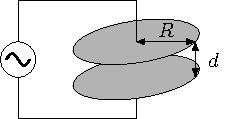
\includegraphics{August2021/3-1.pdf}
\end{center}

\begin{parts}
    \item What is the magnetic field between the plates?

    \item Find the Poynting vector in the space between the capacitor plates.
    What is the direction of the electromagnetic energy flow?
\end{parts}

}

\sol{}


\prob{3.2}{

A point charge $q$ is placed between two perpendicular semi-infinite metallic plates as shown in the figure below.

\begin{parts}
    \item Calculate the electric potential $\varphi(x,y,x_0,y_0)$ produced by the charge.

    \item Calculate the components of the force $F_x(x_0,y_0)$ and $F_y(x_0,y_0)$ acting on the charge as functions of its cartesian coordinates $x_0$ and $y_0$.
\end{parts}

\begin{center}
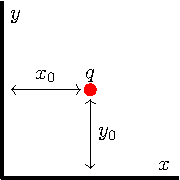
\includegraphics{August2021/3-2.pdf}
\end{center}

}

\sol{}


\prob{3.3}{

\begin{center}
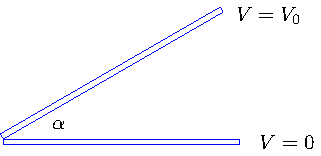
\includegraphics{August2021/3-3.pdf}
\end{center}

Two flat conducting plates form a wedge with apex along the $z$-axis.
The bottom plate is at ground potential and fills the half-plane $y = 0,x > 0$, while the second plate forms an angle $\alpha$ with the bottom one an dis at fixed potential $V_0$.
Solve for the electric potential $V(r,\phi)$ anywhere between the 2 plates, using separation of (cylindrical variables).

\textbf{Hint}: The Laplacian in cylindrical coordinates can be writeen as
\begin{align*}
    \Delta = \pdv[2]{r} + \frac{1}{r} \pdv{r} + \frac{1}{r^2} \pdv[2]{\phi} + \pdv[2]{z}
\end{align*}
Pick the simplest possible solution for the Laplace equation (no Bessel functions needed!) and show it fulfills all boundary conditions.

}



%%%%%%%%%%%%%%%%%%%%%%%%%%%%%%%%%%%
\subsection*{Quantum Mechanics} %%%
%%%%%%%%%%%%%%%%%%%%%%%%%%%%%%%%%%%
\addcontentsline{toc}{subsection}{Quantum Mechanics}

\prob{3.4}{

Two spin-1/2 particles are in the state
\begin{align*}
    \ket{\Psi} = \frac{1}{2} \ket{\uparrow}\ket{\uparrow} + \frac{\sqrt{3}}{2} \ket{\uparrow} \ket{\downarrow}
\end{align*}

\begin{parts}
    \item If you measure the $z$-component of the total spin $S_{1z} + S_{2z}$, what values might you get and what is the probability for each?

    \item If you measure the total spin-squared $\vb*{S}^2$ with $\vb*{S} = \vb*{S}_1 + \vb*{S}_2$, what values might you get and what is the probability for each?
\end{parts}

}

\sol{}


\prob{4.1}{

Consider an infinitely deep potential well of width $a$, i.e., a potential
\begin{align*}
    U(x) = \begin{cases}
        0, & 0 < x < a \\
        \infty, & x < 0,~ x > a
    .\end{cases}
\end{align*}
The initial state of a particle in this well at $t = 0$ is described by the wave function
\begin{align*}
    \Psi(x) = \begin{cases}
        x, & 0 < x < a/2 \\
        a - x, & a/2 < x < a
    .\end{cases}
\end{align*}
Find the probability of finding the particle on the $n^{\rm th}$ energy level, and estimate numerically this probability for two lowest bound states.

Find the average energy $\overline{E}$.

\textbf{Hint}: You may need the sum
\begin{align*}
    \sum_{N=1,\rm odd}^{\infty} \frac{1}{N^2} = \frac{\pi^2}{8}
.\end{align*}

}

\sol{}


\prob{4.2}{

The Hamiltonian for a particle of mass $m$ is $H = \frac{1}{2m}( p_x^2 + p_y^2 + p_z^2 ) + \lambda x$ ($\lambda$ is a constant).

Find $\expval{L_z}$ as a function of time given that, for $t = 0$: $\expval{L_x} = a$, $\expval{y} = b$, and $\expval{p_y} = c$, where $(a,b,c)$ are constant.

}

\sol{}


\prob{4.3}{

Two interacting point particles of equal mass $m$ move along the $x$-axis.
The most general wave function describing this system is $\psi(x_1,x_2)$.
Assume the Hamiltonian for the system is given as
\begin{align*}
    \mathcal{H} = -\frac{\hbar^2}{2m} \pdv[2]{x_1} - \frac{\hbar^2}{2m} \pdv[2]{x_2} + \frac{1}{4} m \omega^2 (x_1 - x_2)^2
\end{align*}

\begin{parts}
    \item What physical system does this Hamiltonian describe?

    \item Show that the following is a solution to the time-independent Sch\"{o}dinger equation:
    \begin{align*}
        \psi(x_1,x_2) = A \exp( i \frac{P}{\hbar} \frac{(x_1 + x_2)}{2} - \frac{(x_1 - x_2)^2}{2 \sigma^2} )
    .\end{align*}

    \item Express $\sigma$ in terms of the other constants given and write down the eigenvalue $E$ of the Hamiltonian for this solution.
\end{parts}

}

\sol{}


\prob{4.4}{

A neutral particle with spin-1/2 and a magnetic moment proportional to is spin is in the eigenstate with the spin parallel to a constant magnetic field $B_z$ applied along the $z$-axis.
Calculate the probabilities $P_{\uparrow}(t)$ and $P_{\downarrow}(t)$ to observe the particle with the spin parallel and antiparallel to $z$ after an additional constant field $B_x$ was applied along the $x$-axis at $t = 0$.

}

\sol{}